% !TEX program = pdflatex
% Obscurity Is Dead --- condensed venue artifact.
% Derivative of paper/main.{md,tex}; do not edit those from this file.
% Page ceiling: 10 pages. If the build emits an 11th page, compress
% before commit (rule defined in docs/prompts/condensed-paper-prompt.md).
\documentclass[10pt,a4paper]{article}

\usepackage[utf8]{inputenc}
\usepackage[T1]{fontenc}
\usepackage{lmodern}
\usepackage{authblk}
\usepackage[english]{babel}
\usepackage[margin=0.95in]{geometry}
\usepackage{microtype}
\usepackage{graphicx}
\usepackage{booktabs}
\usepackage{tabularx}
\usepackage{caption}
\usepackage{xcolor}
\usepackage{csquotes}
\usepackage[numbers,sort&compress]{natbib}
\usepackage{hyperref}
\usepackage{cleveref}
\hypersetup{
  colorlinks=true,
  linkcolor=black,
  citecolor=black,
  urlcolor=black,
  pdftitle={Obscurity Is Dead --- condensed venue artifact},
  pdfauthor={}
}

\graphicspath{{figures/}}

% Tighten vertical rhythm to honour the 10-page ceiling without
% telegraphic prose.
\setlength{\parskip}{2pt plus 1pt}
\setlength{\textfloatsep}{6pt plus 2pt minus 2pt}
\setlength{\intextsep}{6pt plus 2pt minus 2pt}
\captionsetup{font=small,labelfont=bf,skip=4pt}

\title{Obscurity Is Dead --- Proprietary by Design. Open by AI.\\[2pt]
  \large A condensed report on AI-assisted reverse engineering, the
  collapse of the effort gap, and the methodological discipline the
  collapse demands.}

\author[1]{Florian Krebs%
  \thanks{ORCID: \href{https://orcid.org/0000-0001-6033-801X}{0000-0001-6033-801X}.
  Independent researcher (personal capacity). \textbf{Statement of independence}:
  this is a hobbyist project carried out by the author in a personal capacity.
  It is not part of, endorsed by, funded by, or representative of the views of
  any employer, including the German Aerospace Center (DLR / \textit{Deutsches
  Zentrum f\"ur Luft- und Raumfahrt}). The full statement is reproduced verbatim
  in the closing section of this paper; the canonical narrative is in
  \texttt{paper/main.md} \S 9.5.}}
\affil[1]{Independent researcher (personal capacity)}

\date{\today}

\begin{document}
\maketitle

\begin{center}
\fcolorbox{black!40}{black!4}{\parbox{0.92\linewidth}{\centering
  \textbf{Core submission.}\\
  This is the canonical paper of the project (rule~17, \texttt{CLAUDE.md}):
  self-contained, complete on its own, and intended to be read, reviewed, and
  cited without consulting any other artifact. A long-form companion
  (\texttt{paper/main.md} / \texttt{paper/main.tex}) and an open research
  repository extend the evidentiary record --- additional case-study detail,
  complete transcript registries, the redaction policy, the agent-pipeline
  prompts, and the FAIR / F(AI)\textsuperscript{2}R metadata --- and are referenced where a
  reader may want to \emph{go deeper}. They are never preconditions for
  understanding the claims, KPIs, methodology, or limitations of this paper.
  Distribution remains gated on explicit written consent from the author
  (rule~14, \texttt{CLAUDE.md}).
}}
\end{center}

\begin{abstract}
Modern large language models collapse the \emph{effort gap} that has, for a
decade, served as the dominant security model for consumer IoT. Two empirical
case studies --- Spider Farmer BLE controllers and EcoFlow PowerOcean
residential energy systems --- and a third recursive case study of this
paper's own production demonstrate that AI-assisted analysis turns
theoretical protocol knowledge into practical, replicable local integrations
at roughly six to twelve per cent of the manual labour cost. Two further
IoT-Integrator runs (Ondilo ICO Spa V2; Balboa Gateway Ultra) cross-validate
the methodology across an obscurity-vs-authentication spread. The collapse is
genuinely double-edged but it is also asymmetric: it favours integrators over
attackers, at least at present, because verifying an integration against a
live device is cheap while verifying an exploit against a live target is not.
The contribution of the work is not the case studies --- those are largely
prior community work --- but the integration of eight individually unoriginal
practices into a discipline under which AI-assisted research is auditable per
artifact: transcript preservation, verification-status labelling, provenance
maps, mirror discipline between prose and submission source, a recursive
meta-process case study, base-rate-anchored AI disclosure, legal honesty
about authorship, and FAIR alignment as a precondition. Several maintainer
handles, repository paths, device serial numbers, and credentials are
redacted as \texttt{[REDACTED:<type>:<id>]} markers; the register lives in
\texttt{docs/redaction-policy.md} of the long-form companion repository.
\end{abstract}

\section{Introduction: the effort gap and the central thesis}
\label{sec:intro}

The dominant security posture for consumer IoT is not cryptographic but
economic. Proprietary protocols, obfuscated APKs, and undocumented APIs
raise the activation energy of integration high enough that a casual
researcher gives up. We name this implicit defence the \emph{effort gap}
and read it as the de-facto interoperability barrier of the last decade.
The thesis of this paper is that the effort gap has \emph{collapsed
asymmetrically} --- faster for interoperability work, where success is
verifiable against a working integration, than for offensive work, which
still demands target selection, persistence, and operational tradecraft.

\begin{figure}[ht]
  \centering
  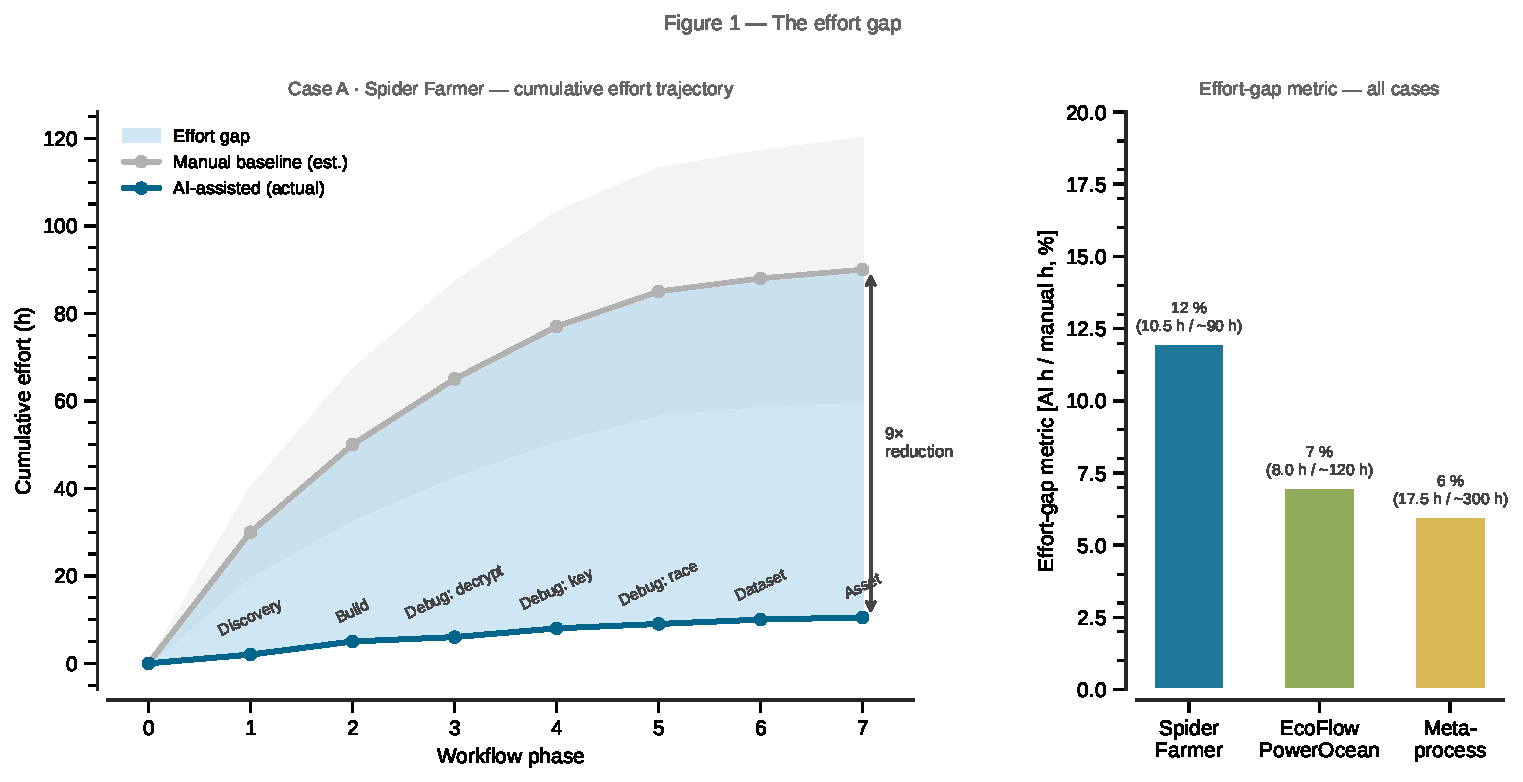
\includegraphics[width=0.85\linewidth]{fig1-effort-gap.pdf}
  \caption{The effort gap. Cumulative human effort to reach a working local
    integration across phases of a reverse-engineering project. AI-assisted
    analysis flattens the curve, leaving a wide effort gap between the two
    trajectories. Source: \texttt{paper/figures/data/effort-gap.csv};
    generation script \texttt{paper/figures/fig1-effort-gap.py}.}
  \label{fig:effort-gap}
\end{figure}

The peer-reviewed software-side anchors are by now consistent: a 24.4\,\%
reduction in cognitive burden when reading AI-augmented decompiler output,
a 31\,\%\,$\rightarrow$\,53\,\% correct-solve rate uplift on
reverse-engineering tasks, and a $>$100\,\% improvement in re-executability
for AI-assisted code synthesis (sources catalogued under cluster~A in
\texttt{docs/sources.md} of the companion repository, IDs L-RE-1 through
L-RE-3). The base-rate evidence on the \emph{defender} side is equally
blunt. Sivakumaran et al.\ found that more than 70\,\% of 17\,243
BLE-enabled Android APKs carry at least one security
vulnerability~\citep{sivakumaran2023bleguuide}; Nan et al.\ statically
analysed 6\,208 IoT companion apps and identified 1\,973 of them, covering
at least 1\,559 distinct vendors, that exposed user data without proper
disclosure~\citep{nan2023iotapp}; Zhao et al.\ measured 1\,362\,906
deployed IoT devices and found 28.25\,\% suffer from at least one N-day
vulnerability, with 88\,\% of analysed MQTT servers having no password
protection~\citep{zhao2022iotbaseline}. Spider Farmer and EcoFlow are not
exceptional cases of consumer-IoT insecurity; they are the median.

The central thesis is therefore that obscurity is dead as a primary defence
for consumer IoT, and that the durable response is \emph{security by design
at the artifact level} --- published specifications, authenticated and
scoped APIs, and threat models that assume the existence of capable,
willing, AI-augmented adversaries. \emph{Full motivation, hardware-side
extension, and contributions list --- see \texttt{paper/main.md} \S 1 in
the companion repository.}

\section{Evidence shape: case studies and headline numbers}
\label{sec:evidence}

The evidentiary base of the paper is four device-integration case studies
(Spider Farmer, EcoFlow PowerOcean, Ondilo ICO Spa V2, Balboa Gateway
Ultra) plus a recursive meta-process case (the paper itself).
Table~\ref{tab:headline-kpi} reproduces the headline-KPI table from the
project README; it is the strongest evidence-shape signal a thirty-minute
reader can take from the paper, and the four-question filter for this
condensed artifact treats it as the load-bearing figure of the section.

\begin{table}[ht]
  \centering
  \small
  \caption{Headline KPI table for the three primary cases.
    \emph{Sources: per-case derivations in the long-form companion
    (\S 3.7, \S 4.7, \S 5.7) and cross-validation rows (\S 6.5).}}
  \label{tab:headline-kpi}
  \begin{tabularx}{\linewidth}{@{}l X X X@{}}
    \toprule
     & \textbf{Spider Farmer} & \textbf{EcoFlow PowerOcean} & \textbf{Meta-process (this paper)} \\
    \midrule
    Defence model & AES-128-CBC keys/IVs hardcoded in APK & 3 undocumented API surfaces; vendor docs cover only~1 & None --- open by construction \\
    AI-assisted effort & $\sim$10.5\,h across 7 transcripts & $\sim$8\,h across 3 transcripts & $\sim$17.5\,h (running) \\
    Estimated manual baseline & 60--120\,h & 80--160\,h & $\sim$300\,h \\
    Effort-gap compression & \textbf{$\sim$12\,\% of manual} & \textbf{$\sim$7\,\% of manual} & \textbf{$\sim$6\,\% of manual} \\
    Live credentials exposed & Yes (MQTT) --- redacted & No (token-bearer) & N/A \\
    Dual-use blast radius & Per-device horticulture control & Grid-in / battery-reserve / EV-charger writes & Fabricated citations, unsourced legal opinions, redaction failures \\
    \bottomrule
  \end{tabularx}
\end{table}

\textbf{Spider Farmer} sealed its BLE protocol with AES-128-CBC under
hardcoded keys and IVs, complemented by a self-signed-certificate MQTT
broker. The AI-assisted contribution was reconciliation rather than
discovery: four prior community implementations agreed on the
cryptographic primitives but disagreed on the dynamic-IV byte range and on
one activation-flow opcode, and the AI pass surfaced the disagreement in
minutes rather than the days a byte-level cross-read of four codebases
would otherwise demand. The case yielded a working Home Assistant
integration plus, as a byproduct, the same live MQTT broker credentials
that an independent community thread had previously recovered --- a
concrete instance of the dual-use signature on which the central thesis
turns. \emph{Full table of cross-implementation reconciliation, key/IV
pinning, and migration narrative --- see \texttt{paper/main.md} \S 3.}

\textbf{EcoFlow PowerOcean} sealed its consumer surface behind three
undocumented API surfaces of which the vendor publishes only one, the
AI-assisted workflow recovering the writeable-parameter catalogue from
APK constants and resolving the three-surface ambiguity in a single pass.
The integration shipped six new writeable Home-Assistant entities (system
reboot, self-check, backup-reserve SOC, fast-charge SOC, charger power
limit, grid-in power limit). The dual-use surface here is non-trivial:
the same controls that enable local automation enable remote
denial-of-availability against a residential energy system. \emph{Full
surface enumeration and type-system bug fix --- see \texttt{paper/main.md}
\S 4.}

\textbf{The recursive meta-process case} treats the paper itself as a
third reverse-engineering target, with the same threat model (fabricated
citations, silent memorisation, prompt injection, AI-generated legal
opinion mistaken for sourced commentary) and the same artifact-inventory
and provenance-map shape as the device cases. Approximately twenty-two
hours of AI-assisted work (rising from seventeen and a half on
2026-05-04 to twenty-two by 2026-05-05) produced the publication-quality
dual-format manuscript, a literature register that grew from seventy
entries on 2026-05-01 to one hundred and forty-four entries across
nineteen clusters by 2026-05-04 and to one hundred and forty-six by
2026-05-05, the FAIR metadata, the redaction policy that govern this
paper, and a public-facing GitHub Pages surface (\texttt{docs/site/})
authorised on 2026-05-05. \emph{Full recursive treatment, transcript
register, and dual-use evaluation --- see \texttt{paper/main.md} \S 5.}

The two further IoT-Integrator runs in \S 6.5 of the long form (Ondilo,
Balboa) are presented in this condensed paper only as cross-validation
and as a useful spread on the obscurity-vs-authentication axis: Spider
Farmer (no auth) $\rightarrow$ Balboa (sound auth, weak operational
layer) $\rightarrow$ Ondilo (clean OAuth2) $\rightarrow$ EcoFlow
(multiple authenticated surfaces). They place the methodology beyond the
original two cases; they do not independently confirm the central thesis.

\section{Method shape: a four-stage pipeline with a ladder underneath it}
\label{sec:method}

\begin{figure}[ht]
  \centering
  
\includegraphics[width=0.9\linewidth]{fig5-methodology.pdf}
  \caption{Methodology. The four-stage pipeline used in every case study:
    Acquire $\rightarrow$ Analyse $\rightarrow$ Audit $\rightarrow$
    Validate, with an explicit feedback loop from validation back into
    analysis. Long-form context in \texttt{paper/main.md} \S 2 and \S 5.}
  \label{fig:methodology}
\end{figure}

Each case study follows the same four-stage pipeline: vendor and community
artifacts are acquired and embedded under
\texttt{experiments/<case>/original/} at a pinned commit; AI-assisted
analysis produces a protocol map or surface enumeration whose every claim
is then audited against the embedded code at the pinned commit; validation
re-runs the smoke test against the live device or, in the meta-process
case, against the rebuilt PDF and the rule-12 mirror parity check. A
feedback loop from validation back into analysis is treated as a
first-class transition rather than as an exception path, because tooling
drift means that an identical prompt at a later date will not produce an
identical output, and the workflow --- not the model's tokens --- is the
reproducible unit.

Underneath the pipeline sits a verification-status ladder applied to every
cited source: an entry progresses from \texttt{[unverified-external]}
through \texttt{[needs-research]}, \texttt{[lit-retrieved]},
\texttt{[ai-confirmed]}, and finally to
\texttt{[lit-read]}, and a paper claim may only invoke a source at the
stage that source has reached. The ladder operationalises the most
concrete and under-managed risk of AI-assisted research, which we name the
\emph{methodological discount}: the unspoken trade-off in which a
researcher accepts a degraded standard of evidence in exchange for
AI-assisted speed. The empirical base rates are severe enough to make the
discount visible --- Walters \& Wilder reported 55\,\% of ChatGPT-3.5 and
18\,\% of GPT-4 generated citations as outright fabricated, with a further
24--43\,\% of the \emph{real} citations carrying substantive
errors~\citep{walters2023fabricated}; McGowan et al.\ found only 2 of 35
ChatGPT-generated psychiatry citations to be real~\citep{mcgowan2023chatgpt};
Chelli et al.\ measured hallucination rates of 28.6--91.4\,\% across LLMs
in systematic-review reference generation~\citep{chelli2024hallucination}
--- and the ladder is the labour-discipline mitigation that no model can
perform on the researcher's behalf.

A redaction discipline runs alongside the ladder and is treated as a
precondition rather than as an afterthought. Several maintainer handles,
repository paths, device serial numbers, and credentials are redacted as
\texttt{[REDACTED:<type>:<id>]} markers in every researcher-authored file;
the full register, the audit trail, and the git-history-rewrite plan that
purges raw values from prior commits all live in
\texttt{docs/redaction-policy.md},
\texttt{docs/redaction-audit-2026-05-03.md}, and
\texttt{docs/git-history-rewrite-plan.md} of the long-form companion. Two
upstream repositories cloned into \texttt{experiments/*/original/} at
acquisition still hold their pre-redaction history and require their own
equivalent passes against the same catalogue before any public-mirror
cut-over. \emph{Full operational methodology, KPI definitions, and
verification-status ladder --- see \texttt{paper/main.md} \S 2; full
redaction register --- see \texttt{docs/redaction-policy.md}.}

\section{Discussion: the eight integrated practices}
\label{sec:discussion}

\begin{figure}[ht]
  \centering
  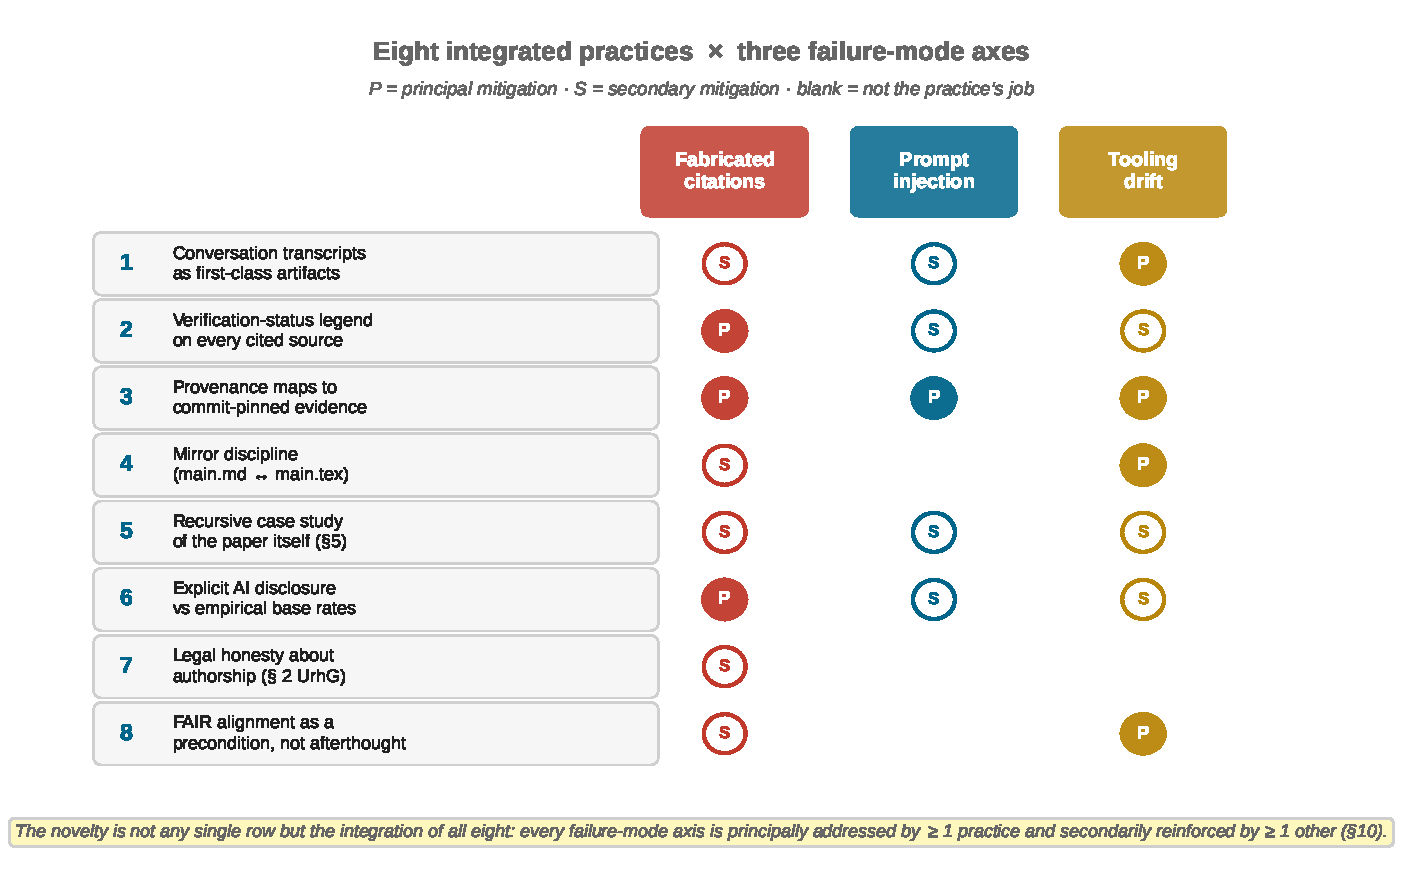
\includegraphics[width=0.9\linewidth]{fig11-eight-practices.pdf}
  \caption{Eight integrated practices $\times$ three failure-mode axes
    (sloppification, model collapse, dual-use). The methodological novelty
    is the integration: every failure-mode axis is principally addressed
    by at least one practice and secondarily reinforced by at least one
    other. Long-form treatment in \texttt{paper/main.md} \S 10.}
  \label{fig:eight-practices}
\end{figure}

The eight practices that organise this paper's methodological contribution
are individually unoriginal --- conversation logs have been shipped with
replications before, verification-status labels exist in
evidence-based-medicine practice, provenance maps exist in bioinformatics,
FAIR predates LLMs --- and the contribution is the integration. They are:
(1) \textbf{transcript preservation} --- every AI conversation that
contributed to a claim is archived verbatim alongside the prose;
(2) \textbf{verification-status labelling} --- every cited source carries a
ladder stage (\texttt{[unverified-external]} $\rightarrow$
\texttt{[needs-research]} $\rightarrow$
\texttt{[lit-retrieved]} $\rightarrow$ \texttt{[ai-confirmed]} $\rightarrow$
\texttt{[lit-read]}) and a paper claim may only invoke a source at its
current stage; (3) \textbf{provenance maps} --- every technical claim is
tied to a transcript, an embedded vendor file/line, and a pinned commit
SHA; (4) \textbf{mirror discipline} --- Markdown prose source and LaTeX
submission source are kept in lock-step so neither can drift unilaterally;
(5) \textbf{a recursive meta-process case study} --- the paper documents
its own AI-assisted production as evidence for the methodology;
(6) \textbf{base-rate-anchored AI disclosure} --- quantitative
fabricated-citation and sloppification base rates are cited inline so the
AI-use disclosure is calibrated rather than rhetorical; (7) \textbf{legal
honesty about authorship} --- AI-generated prose is marked as such;
AI-generated legal opinion is excluded from the paper unless paired with a
sourced primary text; (8) \textbf{FAIR alignment as a precondition} ---
Citation File Format, Zenodo, and CodeMeta metadata are present from day
one rather than retrofitted, with the proposed
\emph{F(AI)\textsuperscript{2}R} extension below (originally proposed as
\emph{FAIR4AI}; renamed 2026-05-05) as an explicit forward direction.

Read as a single discipline, the eight practices cover three failure-mode
axes that the literature makes load-bearing. \emph{Sloppification} is the
proximate corruption of the scientific record by undisclosed AI-assisted
output; the verification-status ladder, transcript-as-artifact discipline,
and base-rate-anchored disclosure address it head-on. \emph{Model collapse}
--- the longer-horizon dilution of the corpus on which future foundation
models are trained, formally argued by Shumailov et
al.~\citep{shumailov2024modelcollapse} and bounded by Seddik et
al.~\citep{seddik2024collapse} --- is the same problem at a
different timescale; provenance maps, mirror discipline, and FAIR
alignment preserve the human-verified ground-truth signal that
mixing-rather-than-replacing strategies require. \emph{Dual use} is the
asymmetry developed below; the recursive meta-process case study, the
redaction discipline (a precondition rather than a practice in its own
right), and legal honesty about authorship operationalise the discipline
that pays for the methodology's openness honestly. \cref{fig:eight-practices}
maps the eight practices against these three axes; worked examples and an
axis-by-axis defence of each cell are in the long-form companion
(\S 10).

The dual-use asymmetry is the most under-discussed feature of the
post-LLM threat model. The same workflow that yields a Home Assistant
integration yields the recovered MQTT credentials and the live device
write paths; the difference between an integrator and an adversary is
governance, not technical capability. Recent evaluations report that
LLMs are far more cooperative than competent at automated exploit
generation --- no model successfully synthesised exploits for refactored
security labs in the L-VD-1 evaluation --- while disclosed-CVE
proof-of-concept generation already reaches 8--34\,\% on public
information alone and 68--72\,\% with adaptive reasoning (L-VD-2), and
the cost-asymmetry literature reports LLM-mediated malicious-content
production at roughly 125--500$\times$ cheaper than human effort
(L-VD-5). \emph{(L-VD-1 and L-VD-5 are recorded at
\texttt{[edge-case]} verification status in
\texttt{docs/sources.md} --- load-bearing, first-of-its-kind,
awaiting human \texttt{[lit-read]} --- and are invoked
here under the verification ladder's edge-case carve-out per
\texttt{CLAUDE.md}, 2026-05-02 extension.)} On 7 April 2026
Anthropic disclosed Claude Mythos Preview, a
frontier model that in their own published red-team work autonomously
identified zero-day vulnerabilities in every major operating system and
every major web browser; the company chose not to release it generally,
instead launching Project Glasswing as a coordinated defensive deployment
and shipping the safeguarded Claude Opus
4.7~\citep{anthropic2026claude} as the broadly-released sibling. The
asymmetry-of-collapse argument is not falsified by Mythos --- verifying
an integration is still cheaper than verifying an exploit --- but the gap
is narrower and the time horizon over which it remains a
defender-favouring asymmetry is shorter than the original framing
assumed. The durable answer is not a better guardrail but security by
design: every guardrail is a classifier, every classifier has a
false-negative rate, and the frame to retire is ``AI is just another
vector''; the frame to adopt is that AI massively increases the
magnitude and frequency of attempts that any given system will face, and
only systems that survive that increase by design will survive at all.

A second strand of skepticism --- that AI-assisted authorship is a
quieter form of plagiarism, and that the methodology defended here is an
elaborate way to launder synthetic prose into the scientific record ---
must be addressed directly rather than dismissed. We take the underlying
claim, that the current default of undisclosed AI assistance is
corrosive, to be substantially correct, and read the eight practices as
our proposal for the conditions under which the legitimate concern is
\emph{answerable} rather than dismissible. The intended move is from
opposition to \emph{co-norm-setting}: disagreement about which practices
belong on the list, which are insufficient, and which the next tooling
cycle will subsume is precisely the kind of engagement we are most hoping
to provoke.

The community already has two adjacent precedents for adapting the FAIR
Guiding Principles to non-data artefact classes. FAIR4RS extends FAIR to
research software, scripts, computational workflows, and
executables~\citep{chuehong2022fair4rs}; FAIR4ML extends FAIR to
machine-learning models and model evaluations~\citep{rda2024fair4ml};
neither yet covers AI-mediated research \emph{processes} --- exportable
conversation transcripts, versioned prompts, tool-and-model version
manifests, verification-status ladders, structured redaction policies. We
propose, as a target for community refinement rather than as a finished
standard, that the eight practices be developed into a \textbf{FAIR for
AI-Assisted Research} extension under the working name
\emph{F(AI)\textsuperscript{2}R} (read \emph{F-A-I-A-I-R}; folds
\emph{(AI)} into the acronym rather than appending an external
\emph{4AI}),
mapping persistent transcript identifiers onto Findability, the
structured redaction policy onto Accessibility, a transcript-export and
prompt-version manifest onto Interoperability, and the combination of
exportable transcripts plus declared tool and model versions onto
Reusability. The repository accompanying this paper already practises
de-facto versions of every element on that list. Naming what we are
already doing, and surrendering it to peer scrutiny before it hardens
into convention, is itself the call-to-action.

\section{Limitations}
\label{sec:limits}

The case base is small and consumer-segment. Four device-integration
cases plus one recursive meta-process case were sampled through
researcher need rather than randomly, and all four are in the residential
/ horticulture / pool-and-spa / energy segments; industrial, OT, ICS, and
safety-critical hardware are not covered. The inference we draw is
correspondingly narrow --- that the \emph{flavour} of the obscurity
barrier (hardcoded keys in mobile companion apps; undocumented REST
surfaces; operational-obscurity at the TLS layer) generalises --- not
that per-device defences are equivalent across segments. Validation
against an industrial case is left to future work.

Validation completeness varies across cases. Spider Farmer and EcoFlow
validation completed against vendor code at commit \texttt{ffdf60c}; the
Ondilo and Balboa runs are \emph{cross-validation} of the methodology
with researcher-side device validation still pending (test checklists
\texttt{T-OND-1..T-OND-10} and \texttt{T-BAL-1..T-BAL-12} recorded in the
per-case \texttt{RESEARCH-PROTOCOL.md} files of the companion repository).
The two newer cases enter this paper as evidence for the methodology's
transferability rather than as end-to-end integration confirmation on the
specific physical devices.

The study's outputs are themselves dual-use. The same artifacts that
operationalise transparency --- pinned APK hashes, weakness tables with
technique tags, runnable smoke tests, executable agent prompts --- are
the inputs an adversarial integrator needs, and the corpus-scale
extension developed in \texttt{paper/main.md} \S 7.14 is feasible
\emph{because} the per-APK cost has collapsed. We accept the asymmetry as
the price of methodological openness; the structural mitigations
(rule-13 redaction policy, dual-use mirror per weakness-table row,
configuration-only Phase 3 outcomes, no public push or Zenodo deposit
without explicit researcher consent under rule 14) raise the cost of
laundering the methodology as an exploit pipeline but do not eliminate
it. The paper does not claim to have solved this problem; it claims to
have made it visible in a form that can be reasoned about and audited.

\section{Conclusion}
\label{sec:conclusion}

AI-assisted reverse engineering does not invent new capabilities; it
lowers the activation energy of capabilities that already existed. The
Spider Farmer and EcoFlow PowerOcean cases show that this lowering is
enough to collapse the effort gap that previously sustained ``security
through obscurity'' as a viable consumer-IoT defence; the Ondilo and
Balboa cross-validation cases place the methodology beyond the original
two; the recursive meta-process case shows the same compression applied
to the production of empirical research itself. The collapse is genuinely
double-edged but it is also asymmetric, compressing the integration path
more aggressively than the offensive path --- for now, and for a horizon
whose length the Mythos disclosure has shortened.

A persistent source of confusion in the public debate, and increasingly
in the academic one, is the conflation of \emph{artificial intelligence}
in the broad methodological sense (the family spanning symbolic systems,
classical machine learning, deep learning, reinforcement learning, and
the present generation of large language models) with \emph{generative
AI} in the narrow sense (the LLM-and-diffusion-model subset that drives
the current hype cycle). The empirical effort-gap collapse documented
here is driven by the generative-AI subset; the broader AI methods
family has been shaping security-research workflows for years and will
continue to do so after the present hype cycle subsides. Norms calibrated
only to the current LLM cohort will age out the moment the cohort does;
norms calibrated to the AI methods family as a whole are the ones we
will still need in 2030.

The empirical moment this paper documents is unusual: the present cohort
of researchers experiences AI-assisted scientific work as a routine
modality rather than as an experimental novelty, and that position
carries the obligation to use the window in which the practice is still
being formed to \emph{generate} the norms of acceptable use rather than
to inherit them, retrofit them, or have them imposed after the fact. The
eight integrated practices are best understood as a \emph{condition
catalogue} for AI-assisted work to be defensible as research --- not a
manifesto, but a checklist whose items can be argued with row by row. We
take the AI-skeptic position seriously and read the eight practices as
our offer to skeptics for whom undisclosed AI use is the principal harm:
a discipline under which AI-assisted work can be evaluated on its own
terms. Disagreement about which practices belong, which are insufficient,
and which the next tooling cycle will subsume is the engagement we are
most hoping to provoke. The candidate F(AI)\textsuperscript{2}R extension above is the
same offer in standardisation form: a name we propose and surrender to
the community.

Obscurity is dead. What replaces it has to be designed, not assumed.

\section*{Statement of independence and personal capacity}
\label{sec:independence}

This work is a hobbyist research project carried out by the author
(Florian Krebs, ORCID
\href{https://orcid.org/0000-0001-6033-801X}{0000-0001-6033-801X}) in a
strictly personal capacity. It is \textbf{not} part of, endorsed by,
funded by, supervised by, or representative of the views of any
employer, including the German Aerospace Center (DLR /
\textit{Deutsches Zentrum f\"ur Luft- und Raumfahrt}). The author's
day-job affiliation is acknowledged here only so the reader can rule it
out: no DLR resources, infrastructure, datasets, or
employer-confidential information were used in the preparation of this
paper or its underlying repository. The author's day-time research at
DLR concerns experimental data management (\texttt{shepard}) and is
unrelated to consumer-IoT reverse engineering. Any opinions expressed
are the author's own. The repository's \texttt{CITATION.cff},
\texttt{.zenodo.json}, \texttt{codemeta.json}, and \texttt{docs/fair.md}
all carry the affiliation \textbf{``Independent researcher (personal
capacity)''} in line with this statement. To preempt confusion: the
author's DLR e-mail address (\texttt{florian.krebs@dlr.de}), where it
appears in DLR-ELIB metadata or in any contact channel that the reader
may reach for clarification, is a \emph{contact channel}, not an
\emph{institutional endorsement} --- the personal-capacity framing in
this section governs.

\section*{Companion / extended evidentiary record}
\label{sec:pointers}

This paper is self-contained --- every claim invoked above is supported
by a citation, a Table~\ref{tab:headline-kpi} row, or one of
Figures~1--3. A reader who wants to \emph{go deeper} into a specific
strand will find the following extensions in the long-form companion
(\texttt{paper/main.md} / \texttt{paper/main.tex}) and the open
repository:
\begin{itemize}\setlength{\itemsep}{0pt}
  \item \textbf{Worked examples and an axis-by-axis defence of each of
    the eight practices} --- long-form \S 10.
  \item \textbf{Transcript registry and provenance matrices} ---
    long-form \S 3.2, \S 5.1; \texttt{experiments/*/provenance.md}.
  \item \textbf{Verification-status ladder} with the
    \texttt{[ai-confirmed]} / \texttt{[lit-read]} carve-outs and
    Source-Analyzer criteria --- long-form \S 5 and \S 6.4; agent
    prompts under \texttt{docs/prompts/}.
  \item \textbf{Pipeline-vulnerabilities discussion for the
    IoT-Integrator agent} (the ``malicious integrator'' scenario)
    --- long-form \S 6.5, \S 7.7, figs~13/14.
  \item \textbf{Full sloppification, model-collapse, and
    fabricated-citation evidence base} with all literature-cluster
    anchors --- long-form \S 7.
  \item \textbf{Redaction policy, history-rewrite plan, and the executed
    \texttt{git-filter-repo} pass} --- long-form \S 5.6;
    \texttt{docs/redaction-policy.md};
    \texttt{docs/git-history-rewrite-plan.md}.
  \item \textbf{Hardware-side effort-gap-compression cluster}
    (silicon, firmware, side-channel) --- long-form \S 1.4 and \S 6.8.
  \item \textbf{APK-mass-probing scenario at corpus scale} --- long-form
    \S 7.14.
  \item \textbf{F(AI)\textsuperscript{2}R mapping} with concrete
    Findability~/~Accessibility~/~Interoperability~/~Reusability cells
    for AI-mediated research processes ---
    \texttt{docs/fair.md}~\S F(AI)\textsuperscript{2}R.
\end{itemize}
These extensions enrich the record but are not preconditions for
understanding the central claims of this paper.

\bibliographystyle{plainnat}
\bibliography{references}

\end{document}
